\section{Compressed Sensing for Radio Astronomy} \label{cs}
A compressed sensing algorithm consists of three components: A Prior, an Objective and an Optimization Algorithm. 

To Include wide field imaging in the objective function directly, which has the potential to improve reconstruction with 
Model the signal to so the reconstruction is plausible
Use an optimization algorithm that is able to handle the expected amount of data. Interferometers produce a large amount of data. In this project, the optimization algorithm was not further investigated. The GuRoBi simplex solver was used.

Compressed Sensing for Radio Astronomy is an active research field. The new instrument's push to wide Field of View imaging has led to increased interest. 

The guarantees in Compressed Sensing depend on the signal, in what space the signal is measured and how well our Prior models the signal. 


\subsection{Sparseland Prior and Incoherence}
From compression algorithm, we assume there is a Prior $P$ in which our signal can be sparsely represented. It is not guaranteed that such a space exists, but for natural signals there always seem to be. This has led to the idea of the Sparseland Prior \eqref{cs:eq:sparseDic}: We assume for our signal there exists a Dictionary $Dic$ of signal parts. There is potentially a large, but finite number entries of parts. When we measure our signal $x$, we see a combination of only a few entries non-zero entries $\alpha$ of the Dictionary. 

\begin{equation} \label{cs:eq:sparseDic}
	\begin{split}
		x = Dic \: \alpha  \qquad  x \in \mathbb{R}^{n}, \alpha \in \mathbb{R}^{m}, Dic \in \mathbb{R}^{n*m}, \qquad n \leq m \\
		\left \| \alpha \right \|_0 = s \qquad s \ll n \leq m
	\end{split}
\end{equation}

Pictures of nature scenes for example tend to be sparse in the wavelet domain. If $x$ in \eqref{cs:eq:sparseDic} are nature scenes, we can create a Dictionary $Dic$ of wavelets. A single image $x$ then consists out of a combination of a few wavelets, meaning the number of non-zero entries is far lower than the number of pixels $n$.

Noise tends to affect all entries of the Dictionary. Sparseland Prior has had success in image denoising.

The signal parts is not restricted to be in one domain. It can consists of wavelets, cosine functions, a combination of both, or any other function. 

Work with over-complete dictionaries, where the number of pixels $n$ is far smaller than the number of signal parts $m$. There are redundant entries which is OK, as long is it is not too redundant. There is a tradeoff in practice in how sparse a signal can be represented and how redundant the dictionary is.

Back to the ill-posed inverse problem of interferometry. Nyquist Shannon Sampling Theorem requires that if we want an image of $n$ pixels, we need at least $2n$ measurements. The small Field of View Interferometer measures complex visibilities, so for $n$ fully sampled pixels we need $n$ complex Visibility measurements.

But when we know it is a Sparseland signal and we know the Dictionary, we could try to measure in the Dictionary space, so we could try to retrieve the non-zero components and only measure $s$ samples. Sadly, this is only possible if we know which entry of the dictionary are non-zero beforehand, which is in general not possible. So we would measure different $\alpha$ and are more likely to hit a zero component. Note however that if we measure a non-zero component of $\alpha$, we learn a lot more about our signal than when we hit a zero component. So the next question is, can we measure in a space where we learn more about the non-zero components of $\alpha$?

Surprisingly, the answer is yes, there is a way. The space in which we measure our signal $x$ should be incoherent from our Dictionary. With that we maximize the amount we learn about the non-zero components of $alpha$ with each measurement. Interestingly enough, constructing an incoherent measurement space is easy: Random projections are very good at being incoherent from the dictionary. 

Random Projections are not possible, the Interferometer measures complex visibilities. Antenna configuration could help. But luckily what also can help is the Wide Field imaging. McEwen \cite{mcewen2011compressed} showed the theoretical improvement on synthetic data.

$P$ in our original objective function. $Dic = P^{-1}$. So if the conversion from image space to Sparseland is only defined when the dictionary is a square matrix. When it has as many signal parts as pixels. The Objective Function can be modified to work with over-complete dictionaries.


\subsection{Objective Function}
L0 norm is not technically a norm. The problem is not convex.

L1 Relaxation of the Objective function
\begin{equation} \label{cs:eq:l1}
\underset{X}{minimize} \: \left \| D_{dirty} - X \star PSF \right \|_2^2 \: + \: \lambda \left \| PX \right \|_1
\end{equation}

The actual CS formulation uses the indicator function for regularization. The indicator function is Zero for each element of $P(X)$ that is also zero, and 1 for each element that is not zero. This objective function \eqref{cs:eq:actual} is not Convex anymore. There are specialized optimization algorithms that minimize the objective \eqref{cs:eq:actual} like Matching Pursuit. 

\begin{equation}
	\begin{split}
		PSF = F^{-1}M
		D_{dirty} &= F^{-1}MV \\
		X &= Dic\:\alpha
	\end{split}
\end{equation}

\begin{alignat*}{2}
	\underset{X}{minimize} \:& \left \| D_{dirty} - X \star PSF \right \|_2^2 &&+  \lambda \left \| P^{-1}X \right \|_1 \\
	\underset{\alpha}{minimize} \:& \left \| D_{dirty} - P\alpha \star PSF \right \|_2^2 &&+ \lambda \left \| \alpha \right \|_1 \\
	\underset{V_2}{minimize} \:& \left \| D_{dirty} - F^{-1} M V_2 \right \|_2^2 &&+ \lambda \left \| P^{-1}F^{-1}V_2\right \|_1 \\
	\underset{V_2}{minimize} \:& \left \| V - M V_2 \right \|_2^2 &&+ \lambda \left \| P^{-1}F^{-1}V_2\right \|_1
\end{alignat*}

All these equations should produce the same result in theory. In practice these different approaches have implications on the model and the chosen optimization algorithm. Not every $D^{-1}$ is defined. Coordinate descent works well on minimizing in the sparse space $\alpha$ directly. Also the convolution has to be explicitly handled when reconstructing in the image space.

L2 norm in the Image space weights more heavily on the lower frequency components.


\subsubsection{Implementation In Casa}
\begin{figure}[h!]
	\centering
	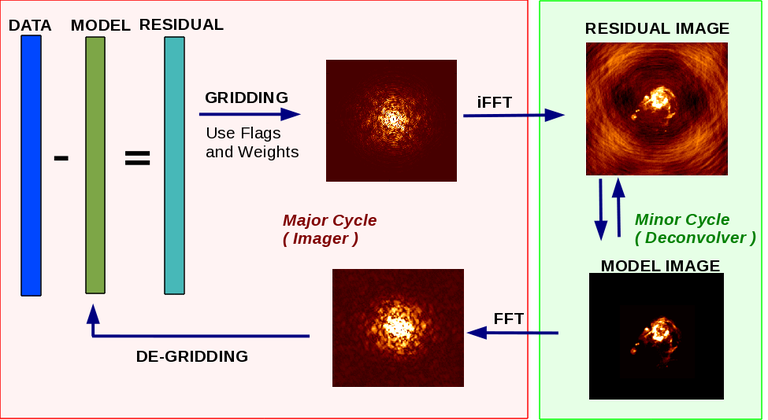
\includegraphics[width=0.6\linewidth]{./chapters/04.cs/img/casa_major_minor.png}
	\caption{Casa Major Minor Cycle, source \cite{casa2018major}}
	\label{cs:major}
\end{figure}

Casa major and minor cycle. Major cycle calculates visibilities in image space. Minor Cycle Deconvolves the Problem, often with a CLEAN class Algorithm. This constrains the algorithm to use the data term in image space. 

This forces the objective function to either minimize in the image domain or in the sparsity domain.


\subsection{Compressed Sensing Algorithms in Astronomy}

\subsubsection{SASIR}

\subsubsection{PURIFY}

\subsubsection{Vis-CS}


 
